\begin{figure}[H]
    \centering
    \begin{subfigure}{1\textwidth}
        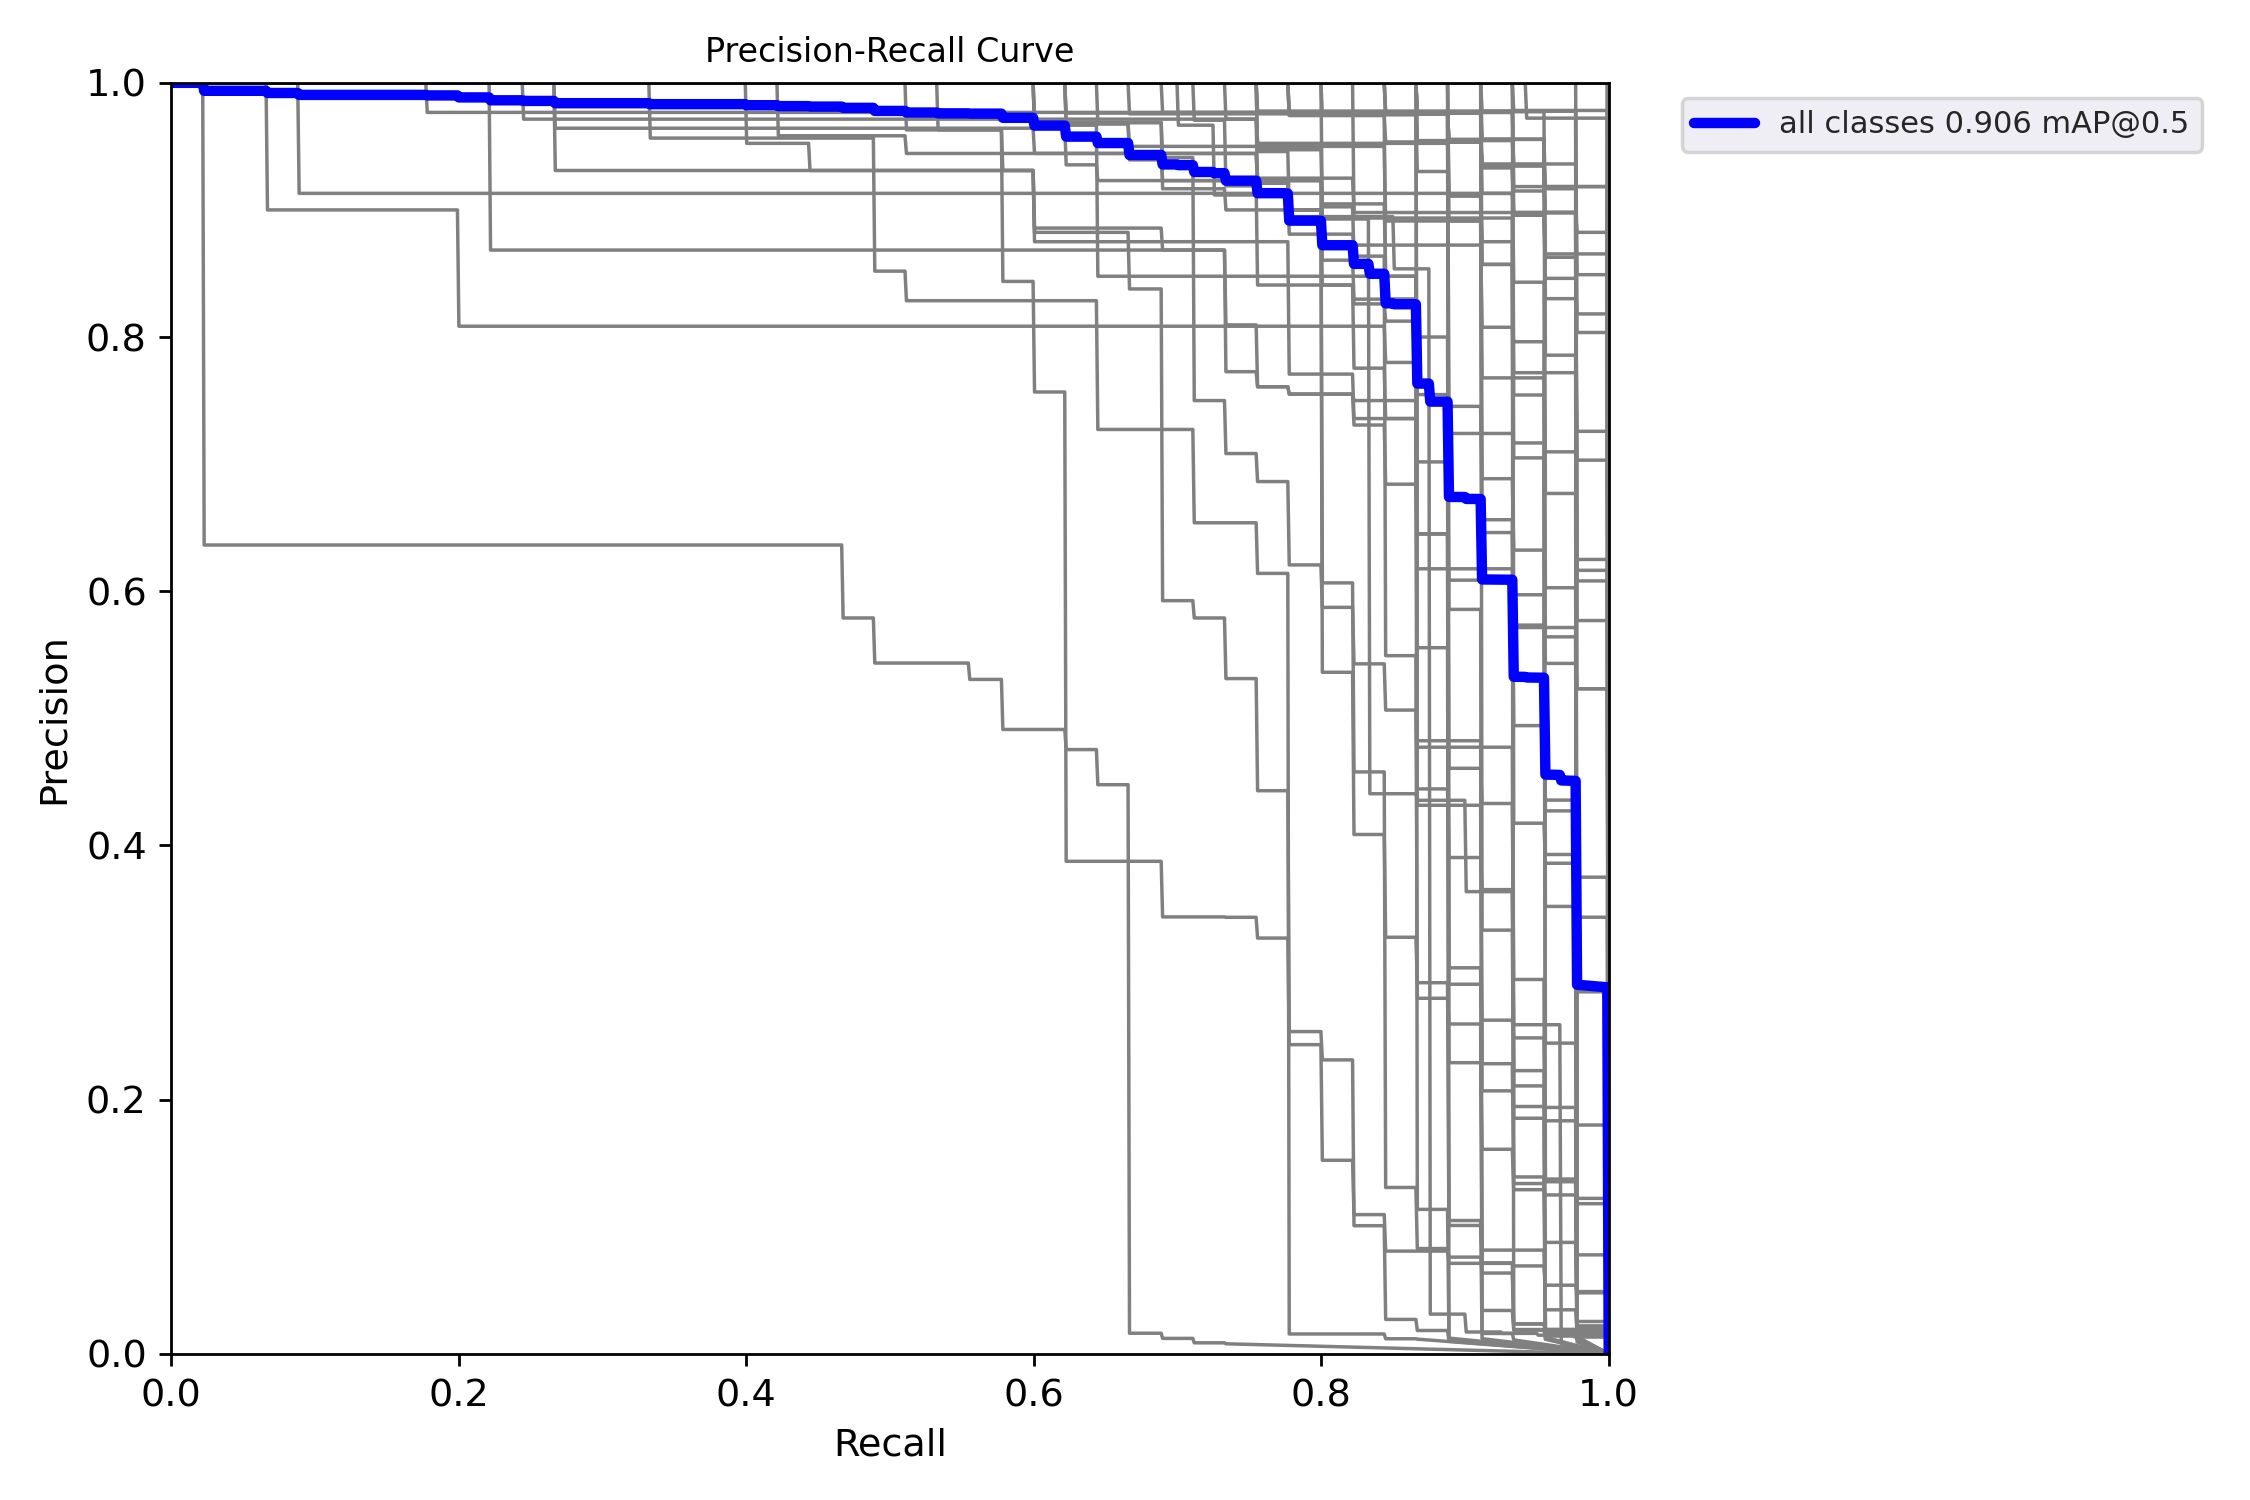
\includegraphics[width=1\textwidth]{images/results/PR_curve.png}
    \end{subfigure}
    \hfill
    \begin{subfigure}{1\textwidth}
        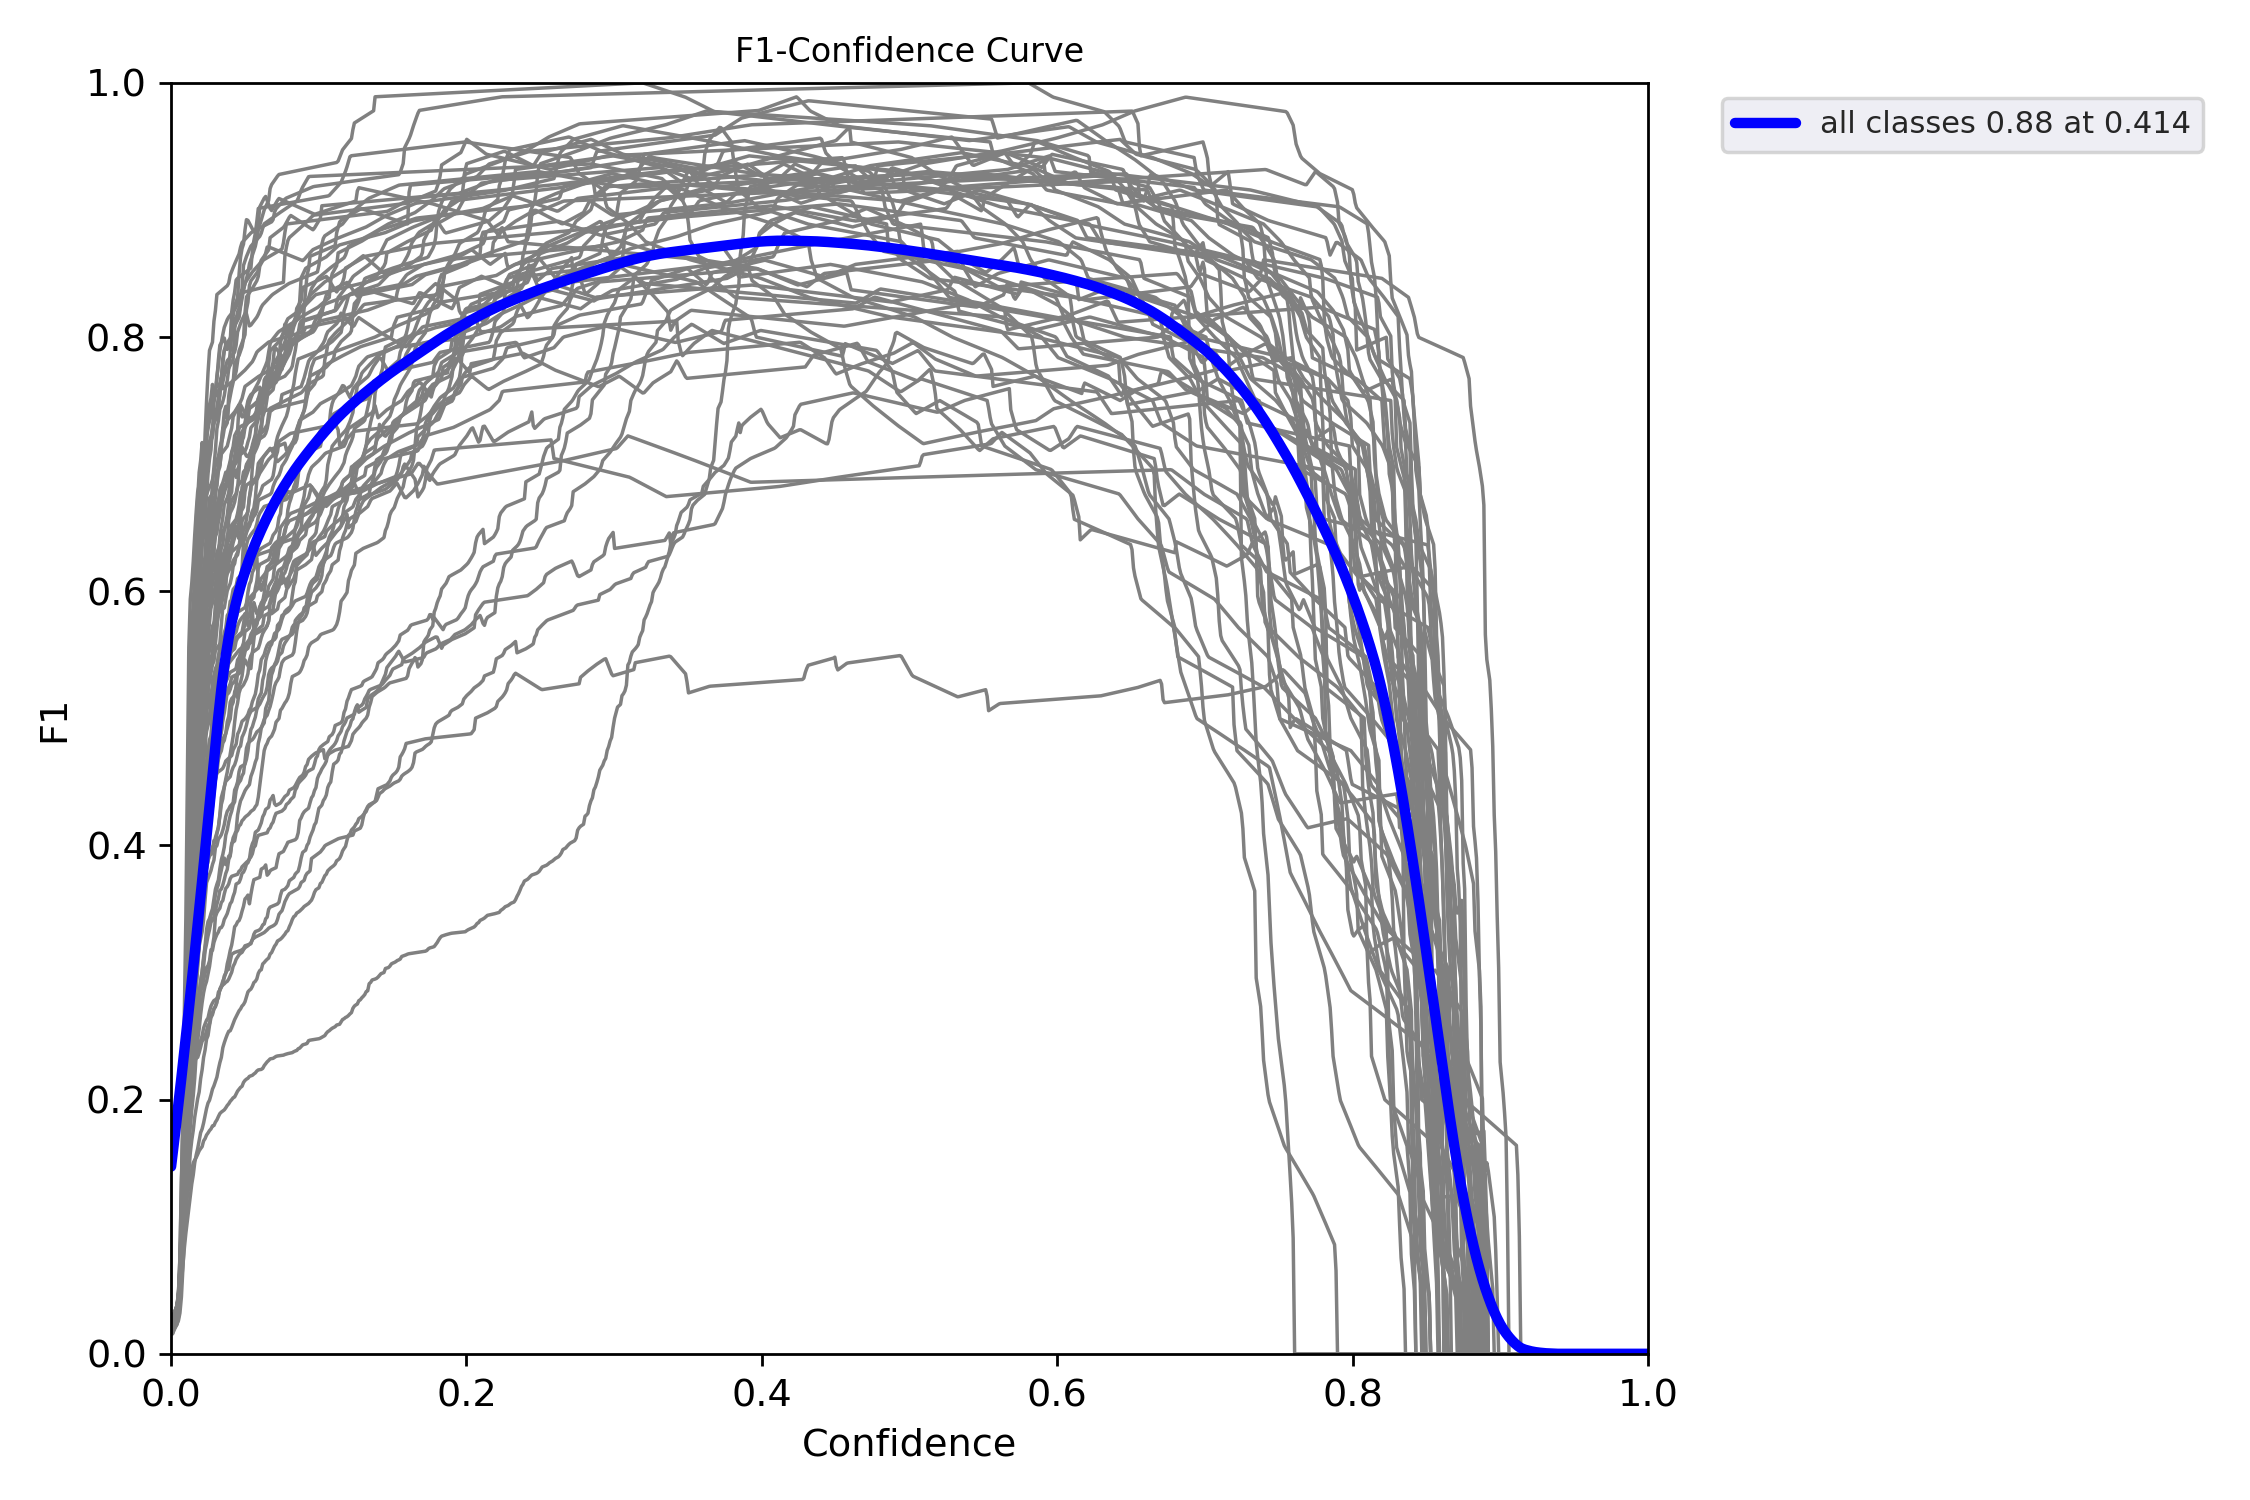
\includegraphics[width=1\textwidth]{images/results/F1_curve.png}
    \end{subfigure}
    \hfill
    \caption{Results}
    \label{fig:result1}
\end{figure}

\begin{figure}[H]
    \centering
    \begin{subfigure}{1\textwidth}
        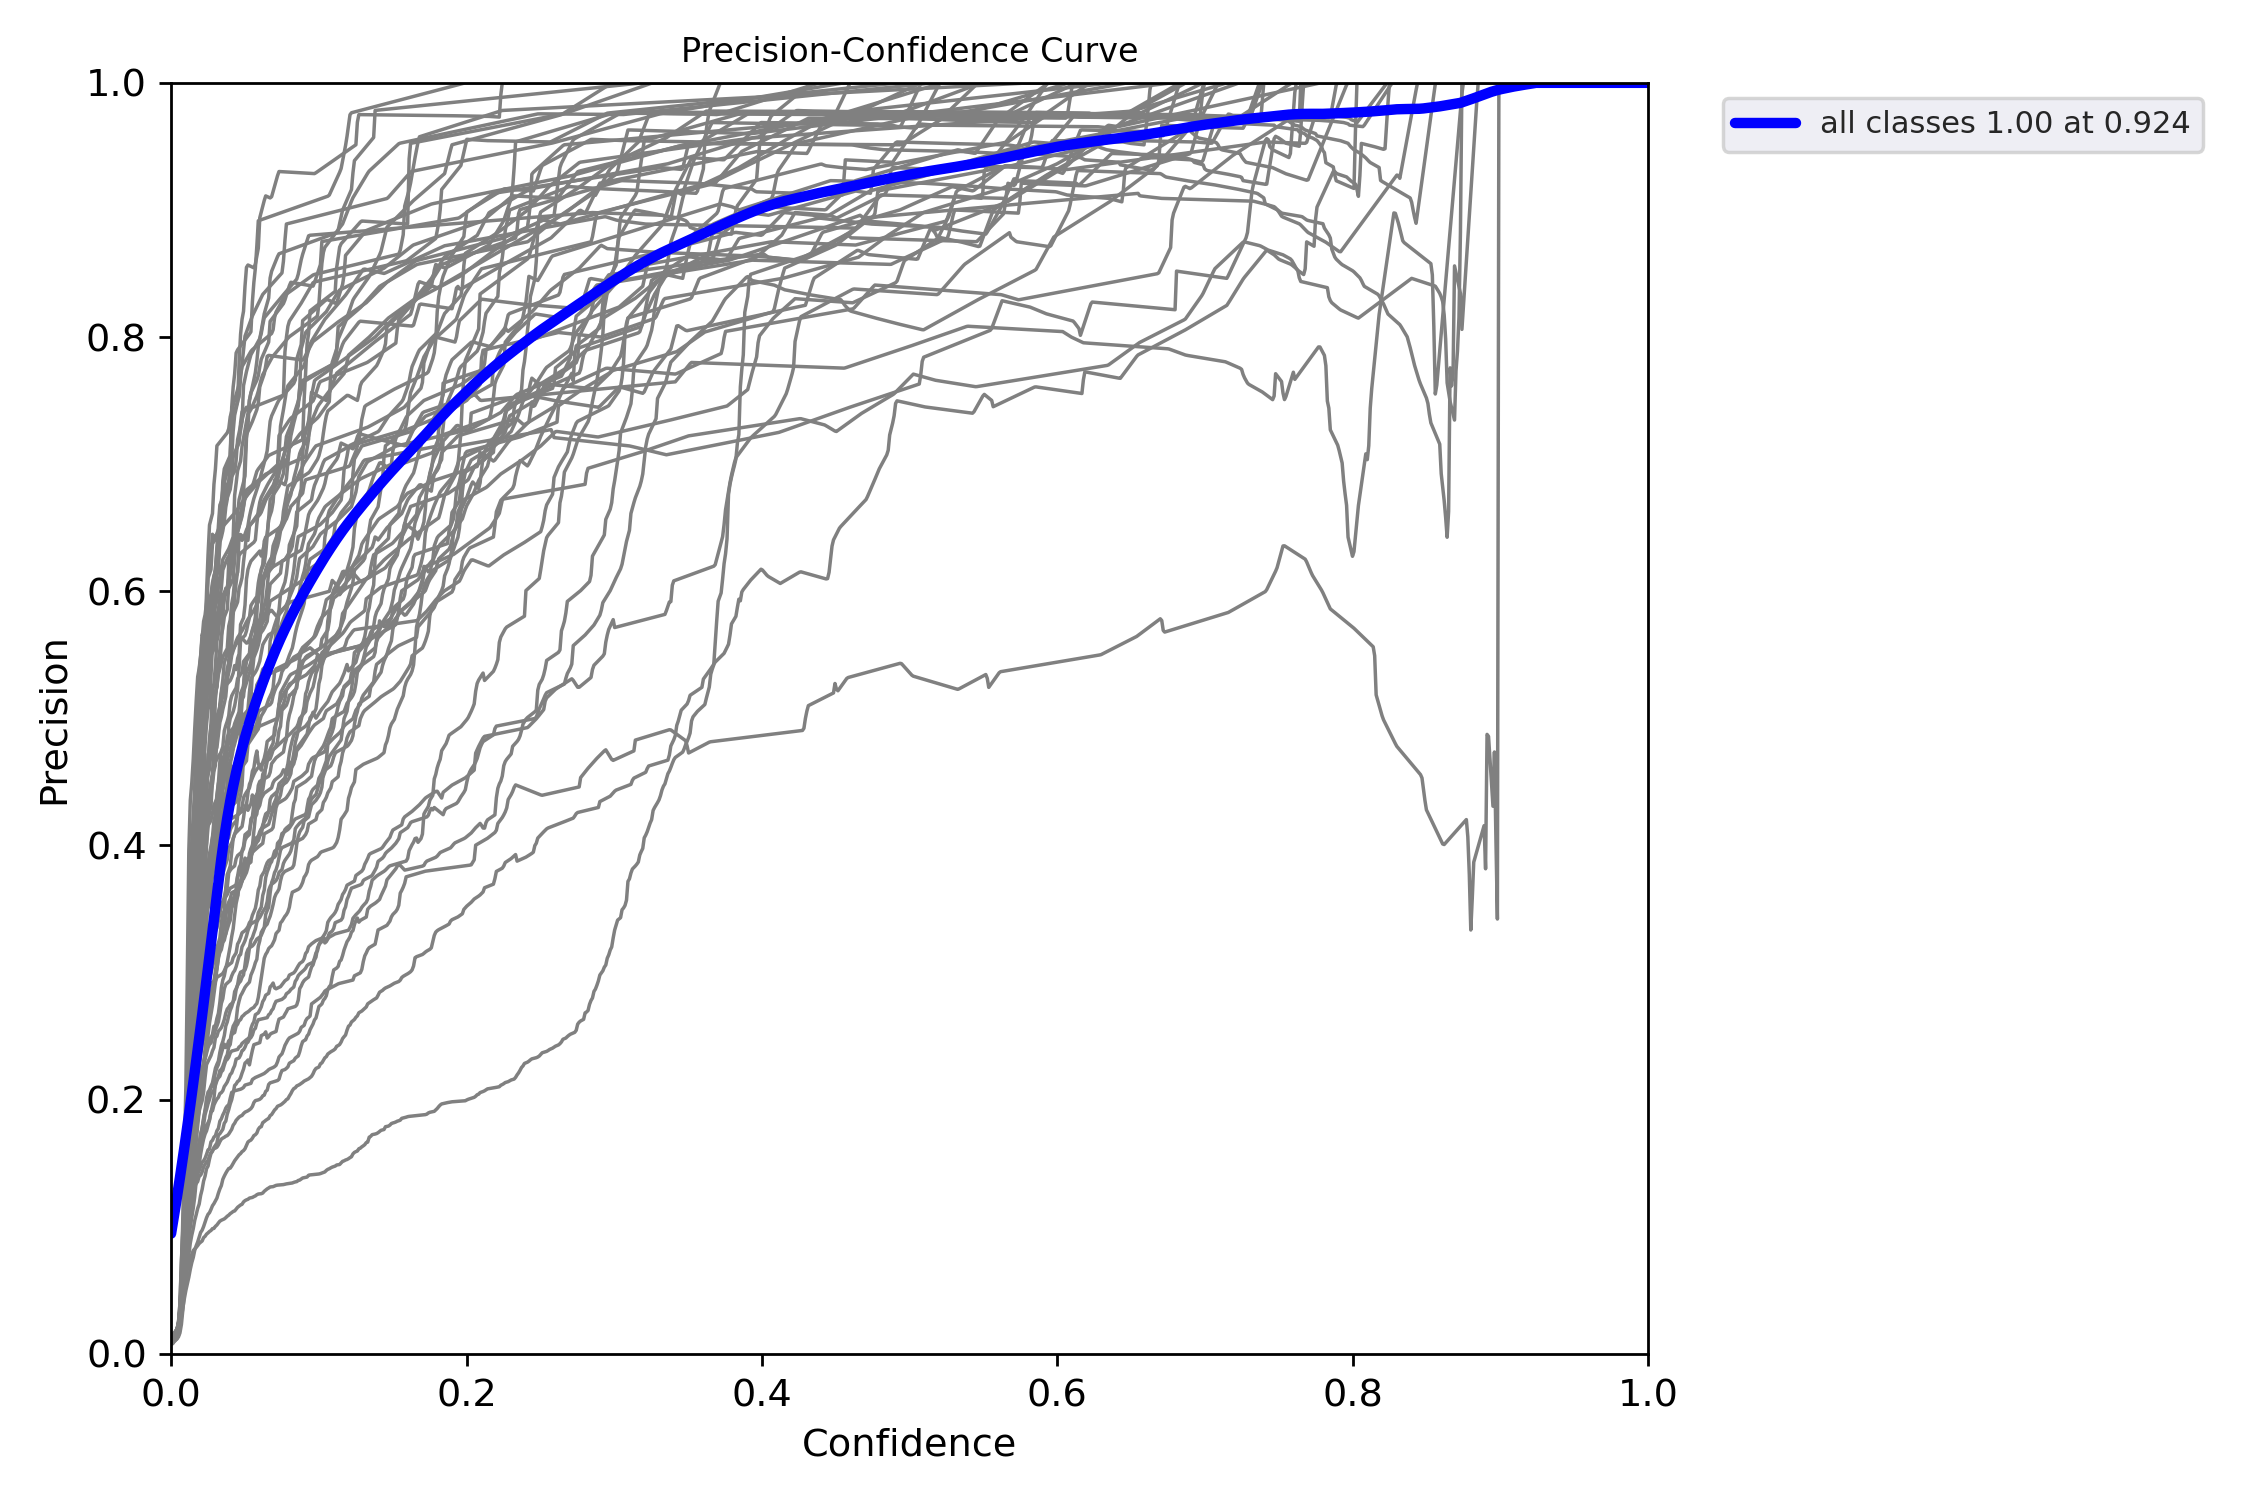
\includegraphics[width=1\textwidth]{images/results/P_curve.png}
    \end{subfigure}
    \hfill
    \begin{subfigure}{1\textwidth}
        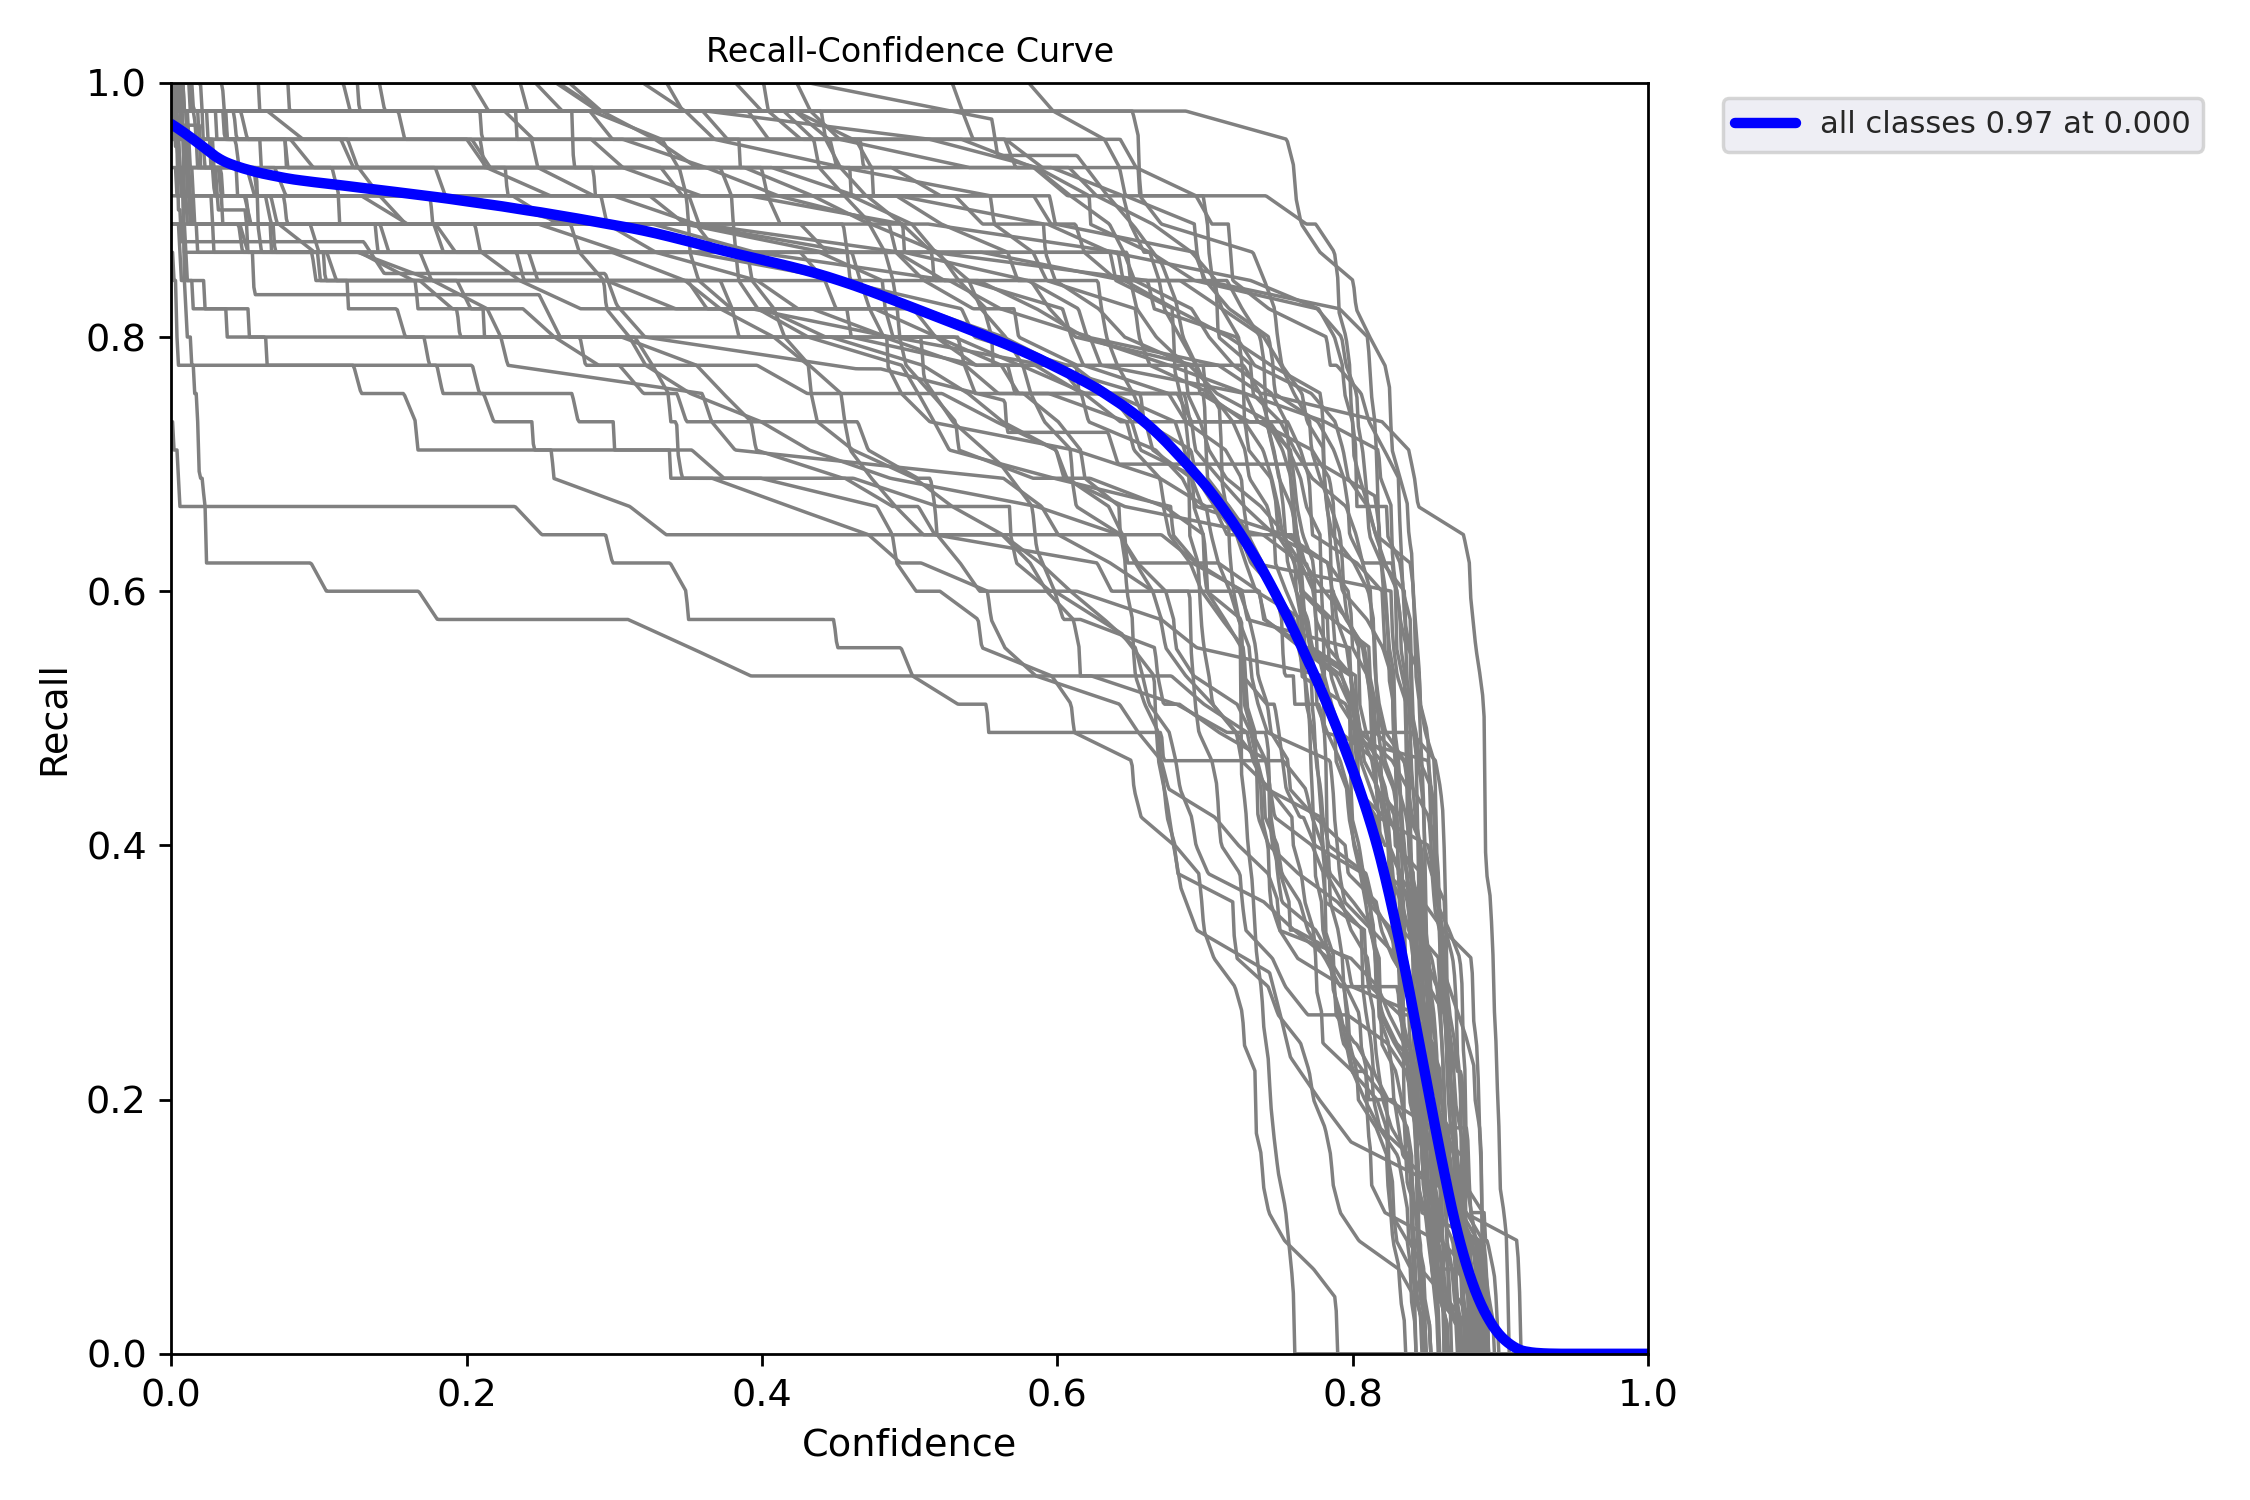
\includegraphics[width=1\textwidth]{images/results/R_curve.png}
    \end{subfigure}
    \hfill
    \caption{Results cont.}
    \label{fig:result2}
\end{figure}

\begin{figure}[H]
    \centering
    \begin{subfigure}{1.1\textwidth}
        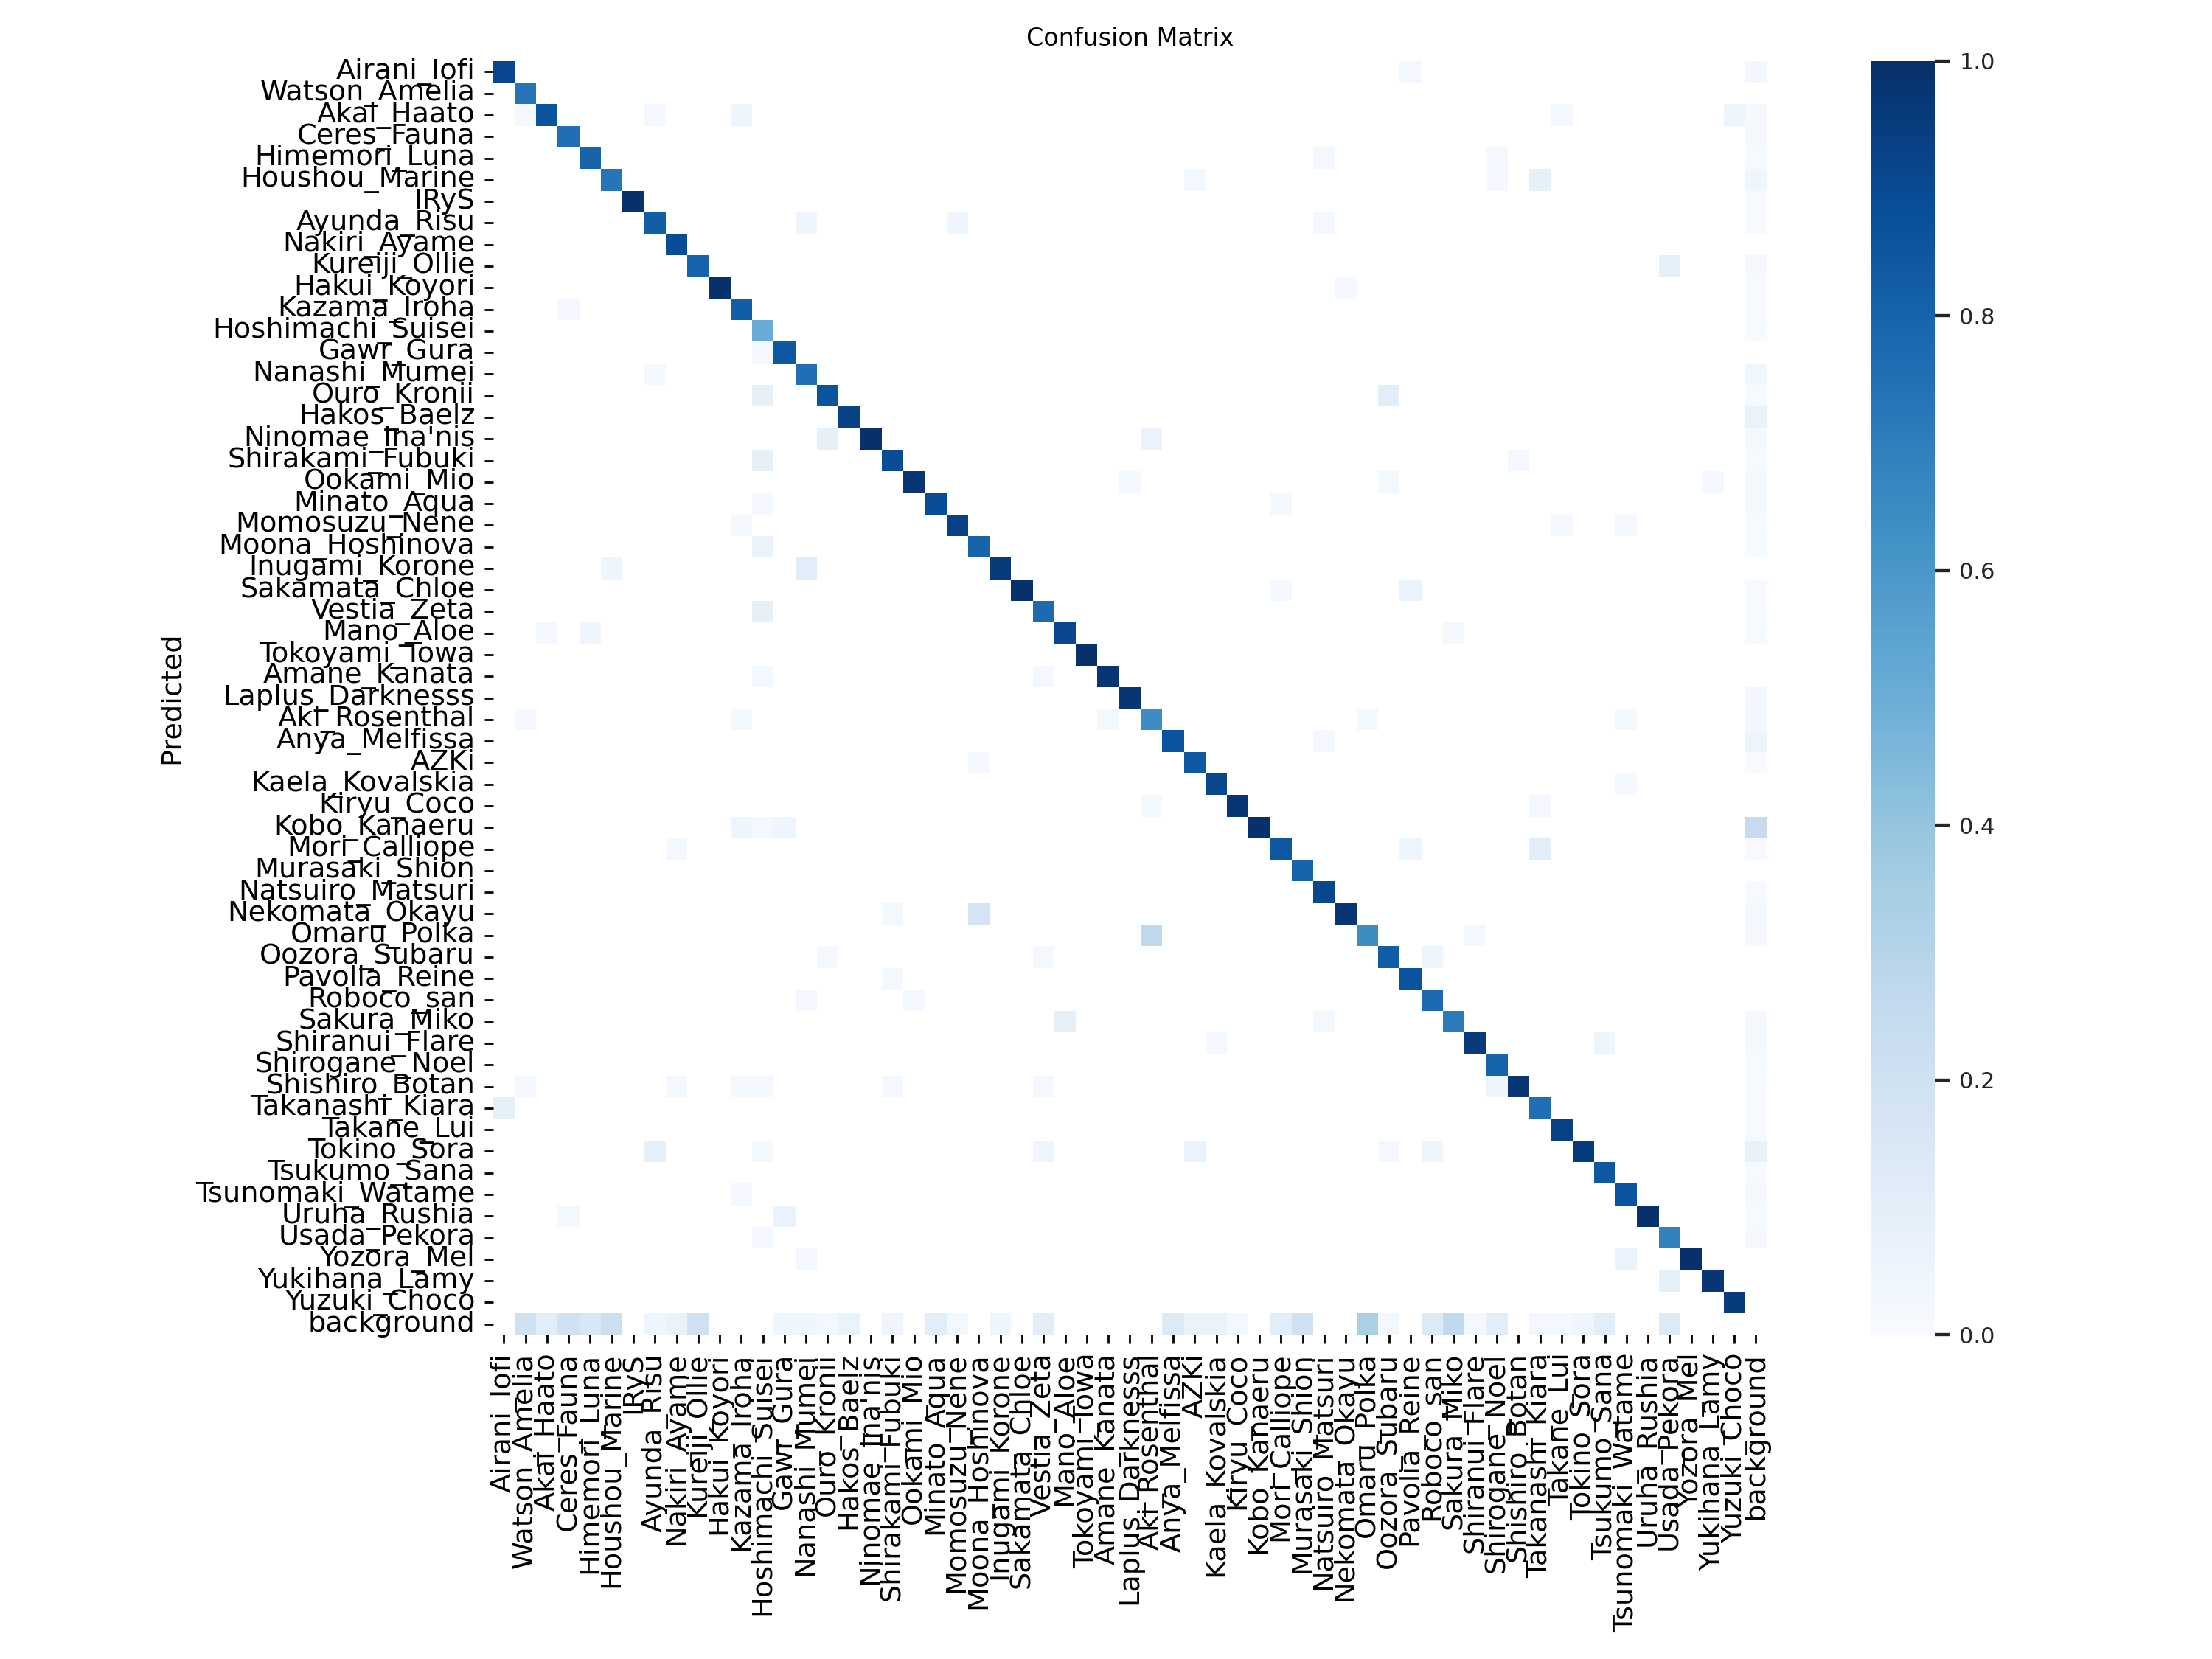
\includegraphics[width=1\textwidth]{images/results/confusion_matrix.png}
    \end{subfigure}
    \hfill
    \begin{subfigure}{1\textwidth}
        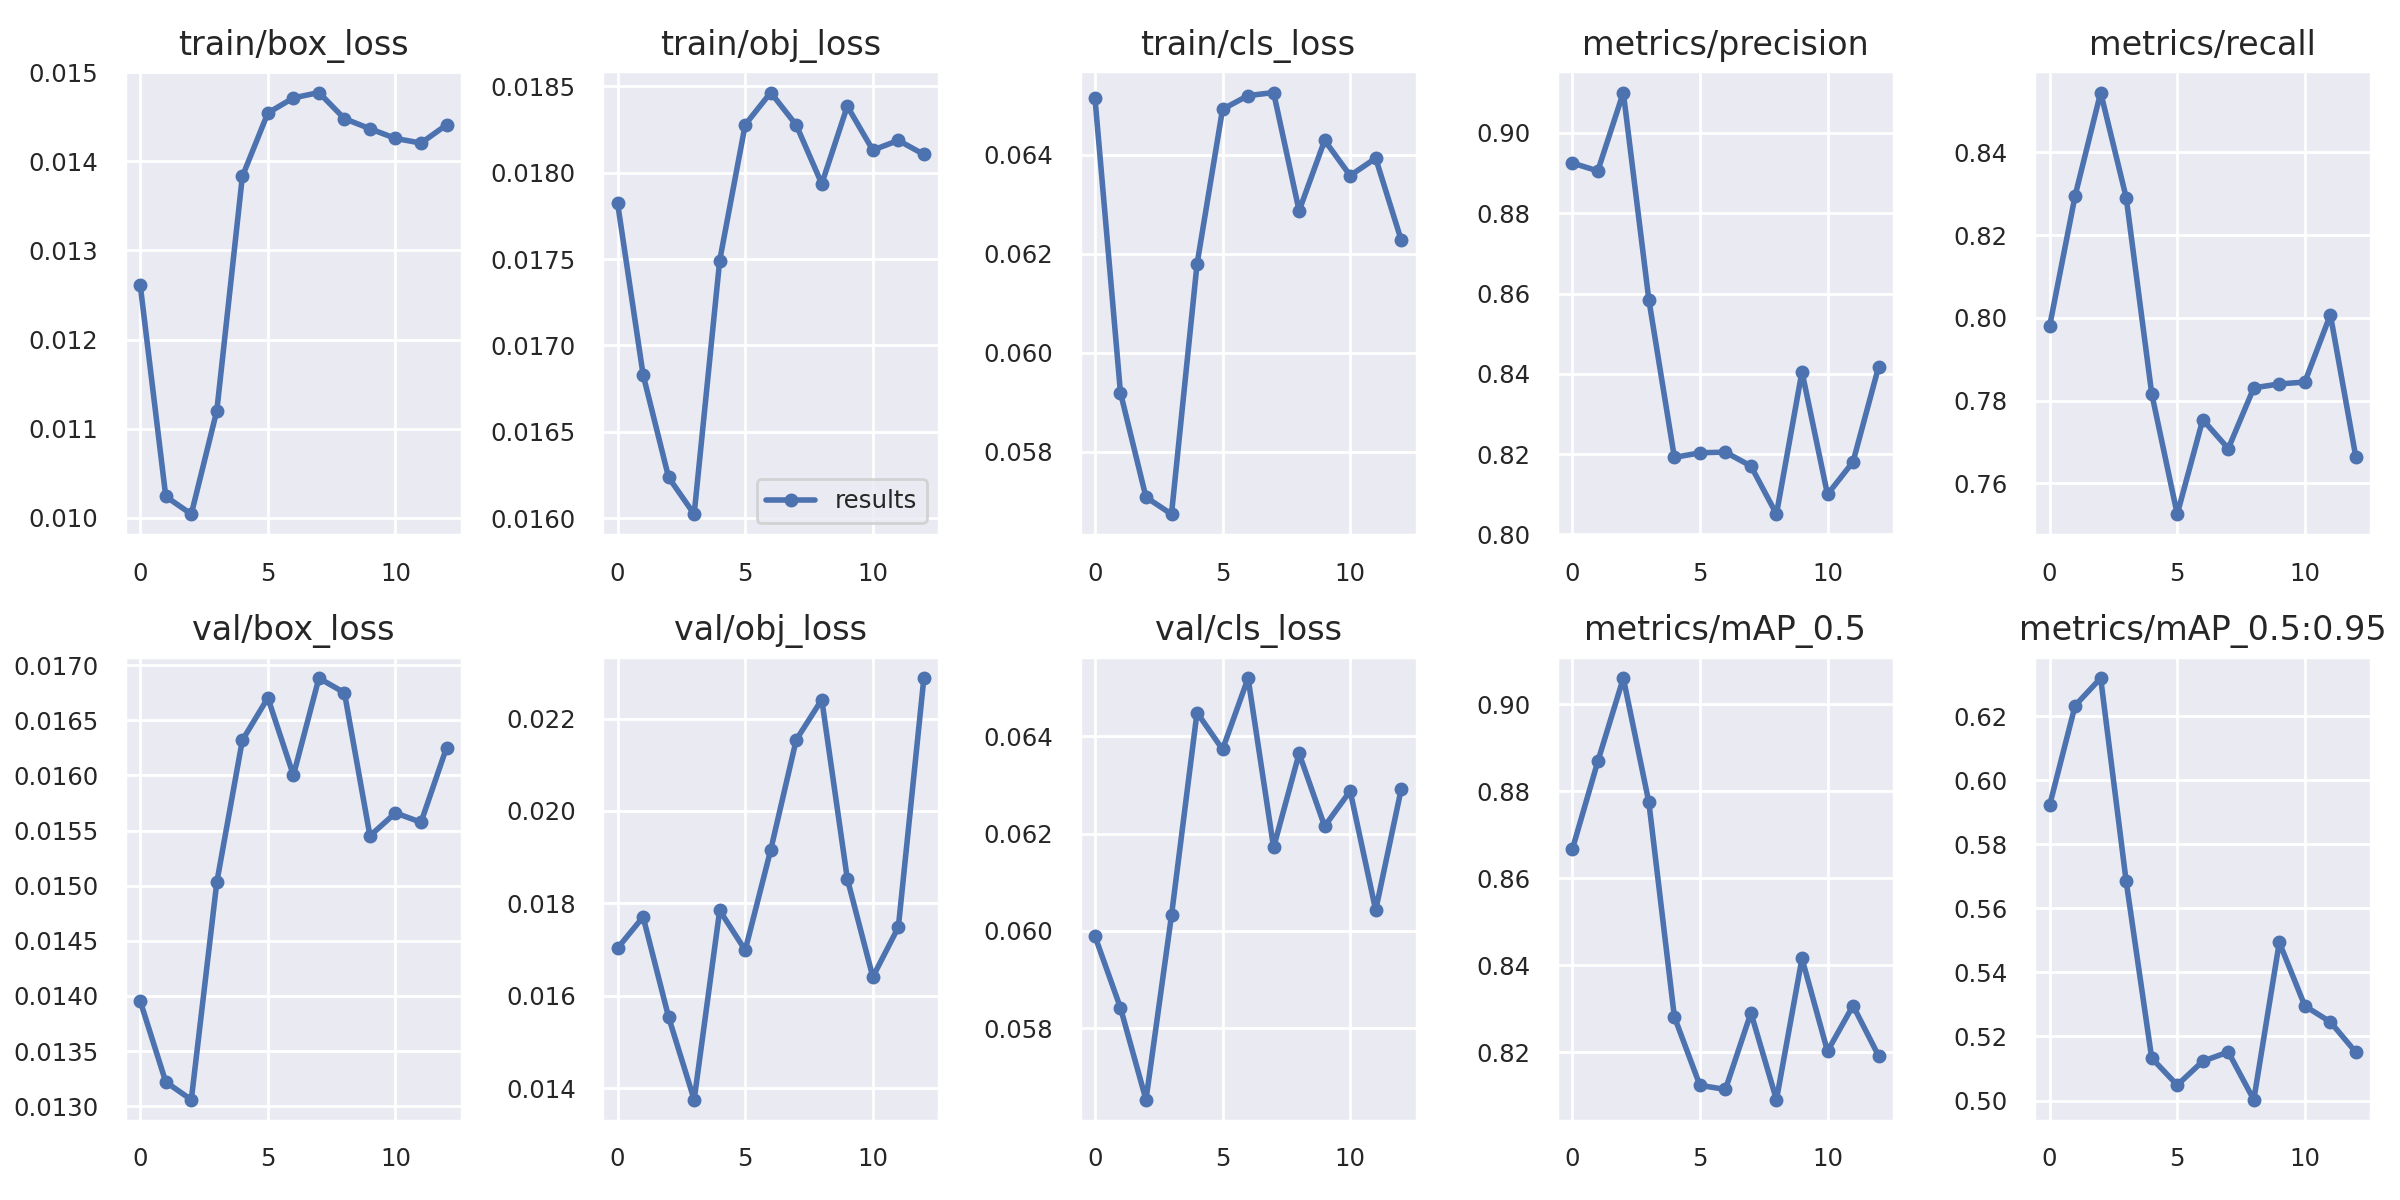
\includegraphics[width=1\textwidth]{images/results/results.png}
    \end{subfigure}
    \hfill
    \caption{Results (cont.)}
    \label{fig:result3}
\end{figure}